\documentclass[pdftex,12pt,letter]{article}
\usepackage[binary-units=true]{siunitx}
\usepackage[margin=0.75in]{geometry}
\usepackage{verbatim}
\usepackage{graphicx}
\usepackage{cite}
\usepackage{color}
\usepackage[pdftex,pdfpagelabels,bookmarks,hyperindex,hyperfigures]{hyperref}
\usepackage{xspace}
\usepackage{amssymb}
\usepackage{authblk}

\bibliographystyle{unsrt}

\newcommand{\fixme}[1]{\textbf{FIXME: #1}}    
\newcommand{\pd}{protoDUNE\xspace}
\newcommand{\dtpc}{\textit{dunetpc}\xspace}

\title{Report from ProtoDUNE Single-Phase Data Challenge 1}
\date{\today}

\author{S. Fuess, A. Mazzacane, R.Pordes, I. Mandrichenko, A. Norman, J.Paley \\
M.Potekhin, G. Savage, H. Schellman, D. Stefan, R.Sulej, S. Timm}


\begin{document}
\maketitle
\begin{abstract}
\noindent We report on the first ProtoDUNE Single Phase Data Challenge that took place in November 2017
\end{abstract}


\begin{itemize}
\item Version 0.1: Initial report draft - missing sections on components still to complete.
\clearpage
\end{itemize}

\tableofcontents
\pagebreak



\section{Introduction and Scope}

The first Data Challenge  (DC1) took place the week of November 6th. The following components were included; 



\begin{itemize}

\item 25 Terabytes of already reconstructed simulation data files from Monte Carlo Challenge 9 were available on EOS at the CERN Tier-0.
In total 28 TB  were copied (some files were copied more than once) using F-FTS-Light running on an OpenStack VM to an EOS data buffer.
From there they were copied using F-FTS to the Data Quality Monitoring dropbox/input buffer, to tape at CERN (on Castor) and Fermilab
(on Enstore) and to disk at Fermilab (dCache). 

\item   The \textit{protoDUNE prompt processing system} (p3s) operated throughout DC1. Its primary goal was to support
the Data Quality Monitoring (DQM)  functionality in \pd by running detector characterization algorithms with a short turnaround time.
The system worked by automatically detecting new input files and running 3 applications on each file: the purity monitor,
noise filtering and event display, and the CRT track matching. 

\item A POMS campaign for processing the files arriving at Fermilab was run in three phases: the first with just the infrastructure
of the current \dtpc to read in and write out the data; the second to .. and the third with the full current payload for the
upcoming protoDUNE-SP MC Data Challenge 10. 

\item In parallel fake data was loaded into the IFBEAM Beam Instrumentation database and existing LHC Beam Line data was ingested into IFBEAM by transfering data from CERN.

\item An initial attempt to run a user \dtpc job using the  usual project.py interface to running grid jobs at Fermilab was
attempted using the site CERN (Tier-0) and a data file stored in Castor provided to the job locally (i.e.~without transferring
the data back from Fermilab to the CERN EOS). 

\item Information about output displays and web pages, monitoring web pages and information, was collected on the wiki.dunescience.org

\end{itemize}

 Fig.\ref{fig:dependencies} shows the components of the end-to-end system and their dependencies. Fig. \ref{fig:intermediate} shows those components included in the Data Challenge. 


\begin{figure}[tbh]
  \centering
  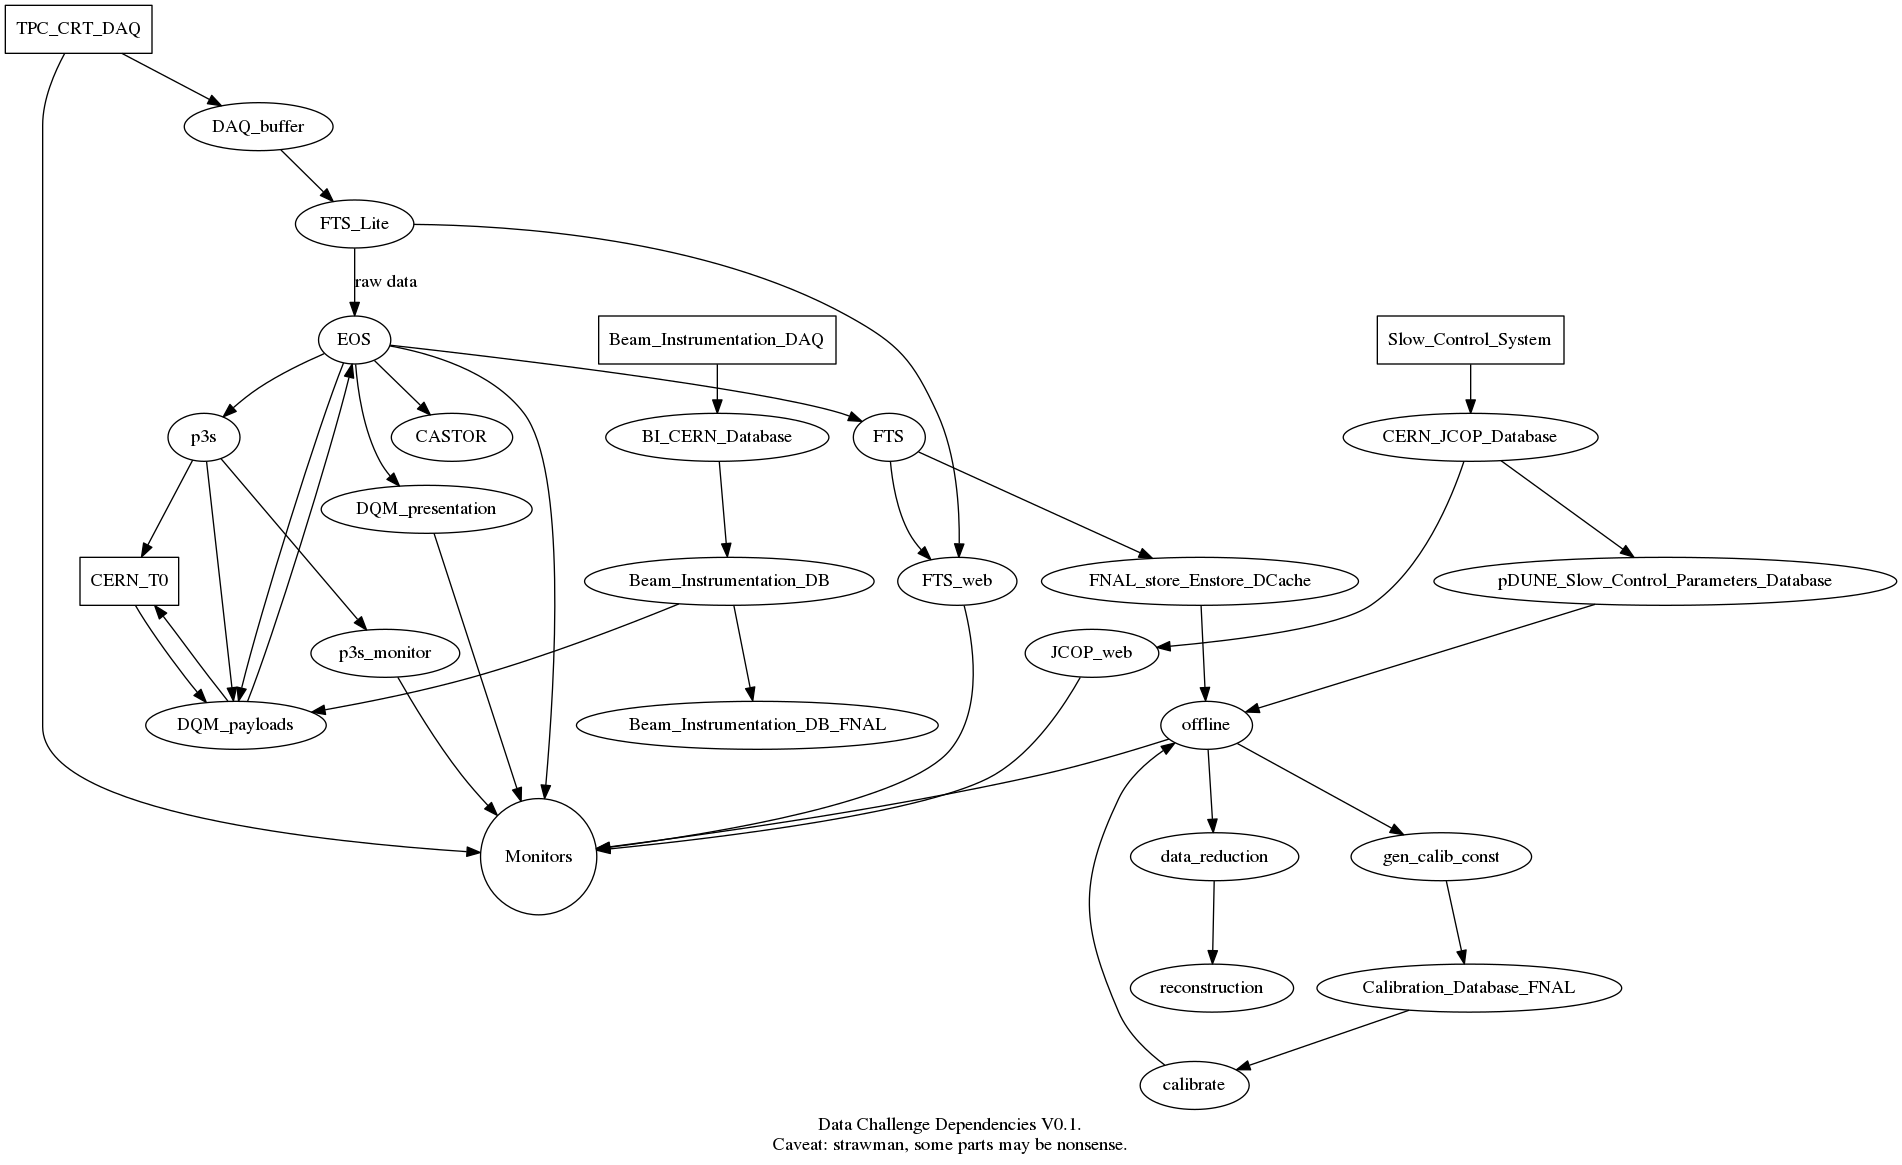
\includegraphics[width=0.75\textwidth]{../figures/dc1_integration.png}
  \caption{Schematic of Dependencies}
  \label{fig:dependencies}
\end{figure}


\begin{figure}[tbh]
  \centering
  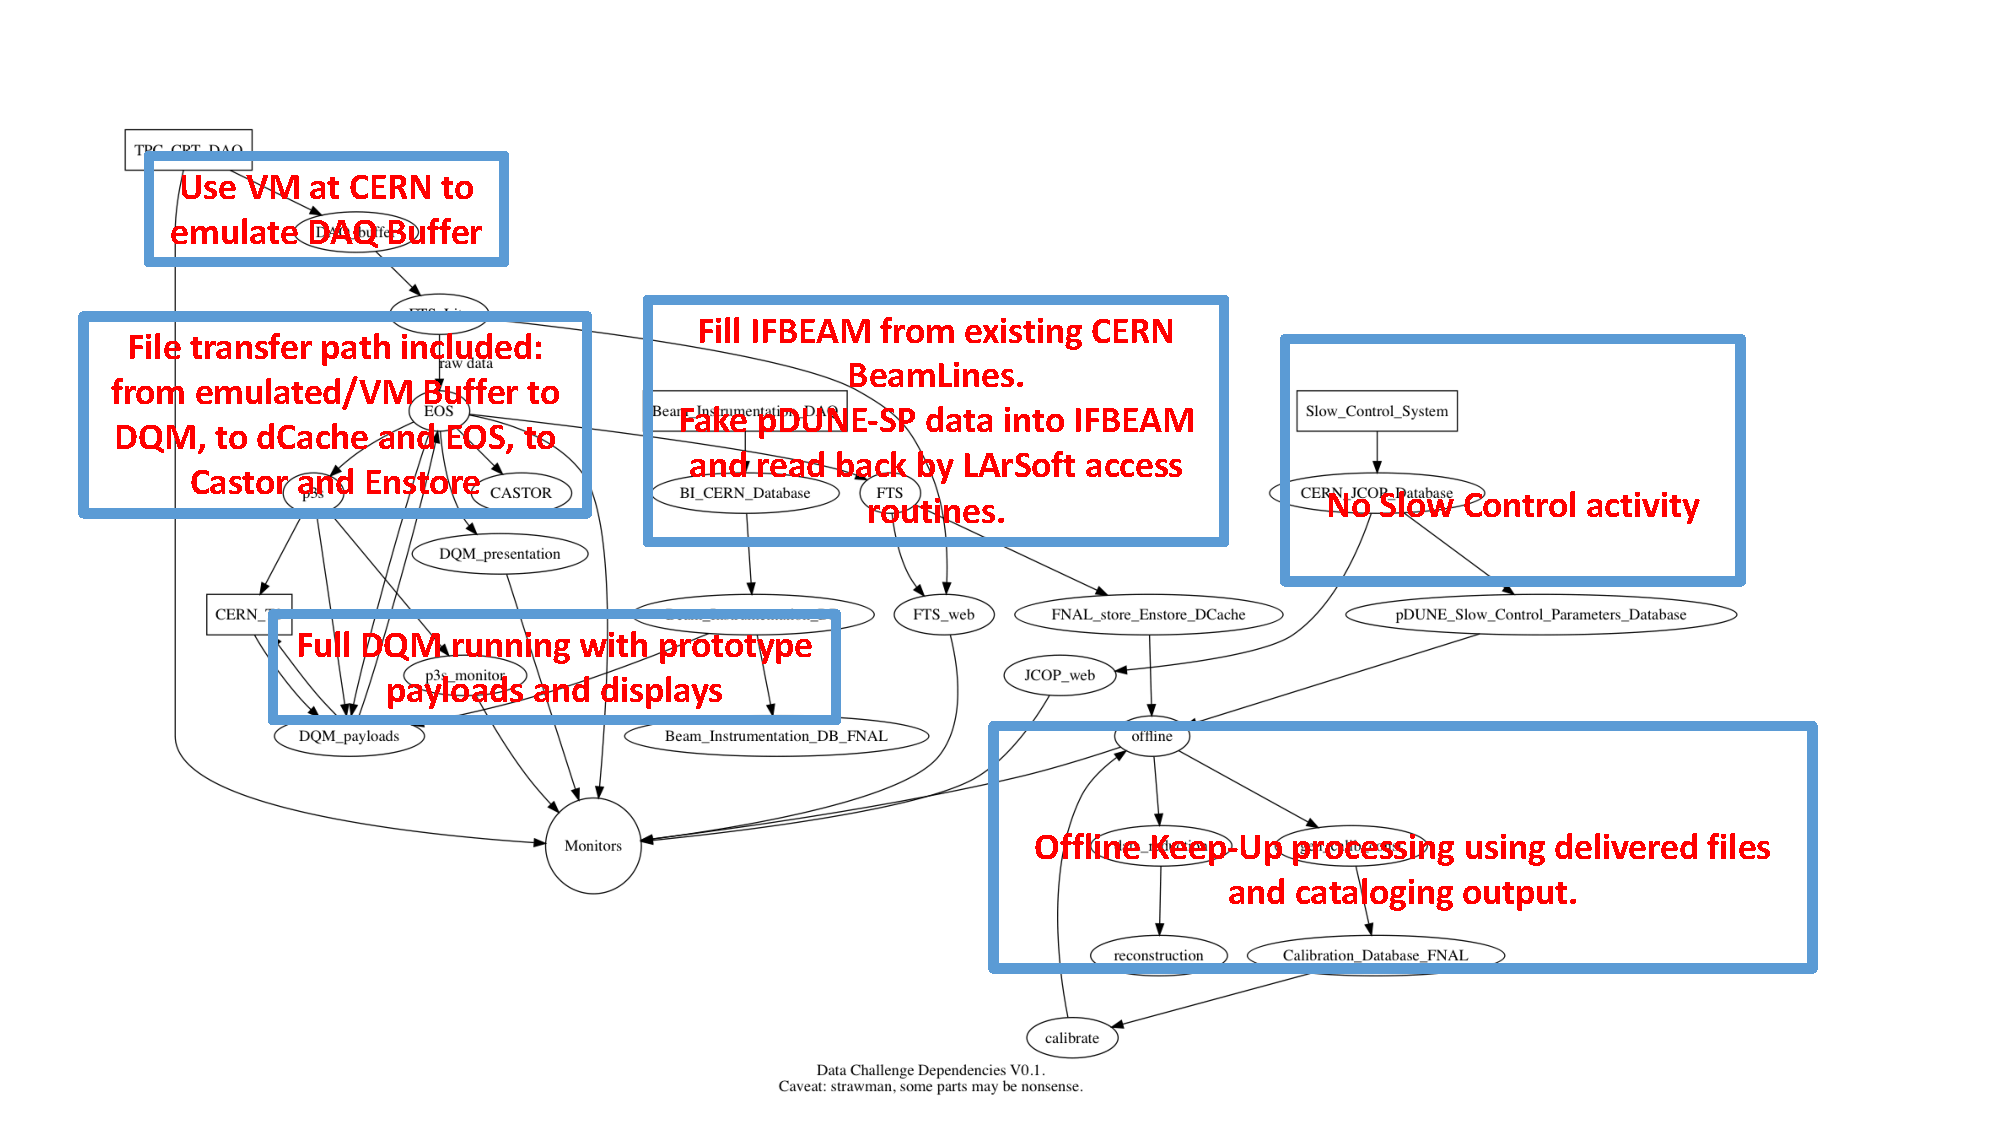
\includegraphics[width=0.75\textwidth]{./ReportImages/intermediate.pdf}
  \caption{What was included in the Data Challenge 1}
  \label{fig:intermediate}
\end{figure}

The groups running each of the components  used in this data challenge analyzed  the latency, throughput and robustness of their software and services together with debugging and identifying problems and solutions. 

Much progress was made during the week that  will stand in good stead for ramping up the whole system to the full data rate and sustainability needed for commissioning and beam running in 2018. 



\section {Data Movement}
\subsection {Definitions}
F-FTS refers to the Fermi File Transfer Service, the standard Fermilab utility which is used to transfer files from a DAQ system to permanent storage and declare them to SAM (Sequential Access with Metadata) database.  F-FTS-Light is a similar program but can operate behind a private net or firewall and does not need to be in contact with SAM or anything else at Fermilab.

The event data used was the dataset of MCC9 data set already available on disk at the CERN EOS, which consisted of
23TBytes,  ~3000 files of average size 8GB, with the data being in  "mergeana" (post merging/processing)  format. There were 
40 subdirectories each corresponding to a different beam energy and with or without space charge effect.

\subsection{Initial Copy Script Details}
From the original location of the MCC9 file  an initial copy script (copy\_mcc9\_data.py): took the files to the simulated DAQ buffer in the EOS file cache via 3rd party xrdcp; added a process ID and a timestamp to the filename; and was configured to ensure a maximum rate at which the xrdcp happened at some point doing the test. It also created a rudimentary set of metadata,

The script could also be configured to stagger copies of files for N seconds between each one or be asked for a specific  count of files. As part of the copy new (SAM) metadata was created. This initial copy broke the 40 directories into 4 chunks and copied 10 directories at once into the buffer, for the goal rate of 500MB/s. As a side-product the test ended up twice launching 5 copies of the copy script rather than one, so 50 xrdcp commands were going at once on the first two days of the DC. This all worked fine with nothing breaking down. See Fig.\ref{fig:EOStoEOS} for monitoring information of the copy. 


\begin{figure}[tbh]
  \centering
  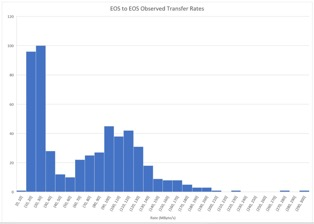
\includegraphics[width=0.5\textwidth]{./ReportImages/EOStoEOS.jpg}
  \caption{EOS to EOS Copy Monitoring}
  \label{fig:EOStoEOS}
\end{figure}

\subsection{F-FTS and F-FTS-Light Operation}
From the emulated DAQ buffer in EOS, F-FTS-Light was used to transfer files into the F-FTS dropbox which was also in EOS.  F-FTS-Light also used 3rd-party xrdcp as its means of file discovery and transport.  It transferred the file, received the checksum that was returned from the xrdcp command, and then added it to the metadata.  Throughout the course of this challenge, F-FTS-Light was configured to transfer 10 files in parallel.   When 10 copy scripts were running upstream, F-FTS-Light was able to keep up to that data flow.  For this test F-FTS-Light ran on an OpenStack VM with 2 cores.  It will eventually run on a server in EHN-1.

For the purposes of this test F-FTS was configured with three destinations:  the input dropbox of the prompt processing P3S, which was also in EOS, Castor tape servers, and dCache/Enstore at CERN.  F-FTS also runs on an OpenStack VM.
For the EOS-to-EOS copy and the EOS-to-Castor copy, 3rd-party xrdcp was used.  For the EOS-to-Fermilab copy we used 3rd party gridftp (globus-url-copy).
FTS was configured to make 10 transfers in parallel to each of the three destinations. Files were declared to the dc1\_input data set in SAM.



\subsection{Results and Observations}
The full set of data files was moved to the 2 archival facilities over the period of about 5 days.  This included gaps of several hours during each day when we did not start any new copies. There were a variety of throughput rates sustained. Changes in configuration of the CERN EOS interface helped with stability of the scripts/services being run. 

On the CERN side an aggregate rate of 200MByte/s was sustained. FTS-Light kept up with the input files, which means it can also handle sending at that rate from the detector. (These rates can be increased by adding more xrdcp processes as needed). Individual file transfer rates show a bimodal distribution due to the fact that some files are stored at Wigner and some at Meyrin.  See \ref{fig:FTSLite}


\begin{figure}[tbh]
  \centering
  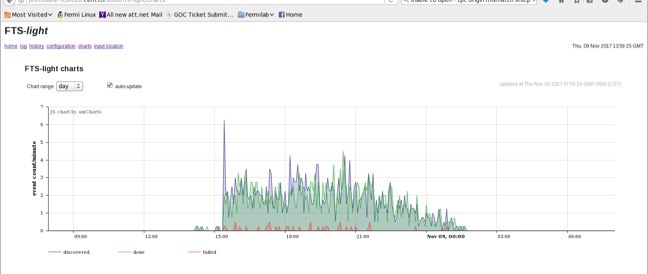
\includegraphics[width=0.5\textwidth]{./ReportImages/FTSLite.jpg}
  \caption{FTS Lite transfer monitoring}
  \label{fig:FTSLite}
\end{figure}


On the CERN Tier-0 the monitoring showed that the EOS traffic generated clearly dominated the EOS accessed during the time of the tests without crashing any EOS servers. (For short periods the monitoring showed that the EOS can even take much higher influx and then recover.)

For the transfers from CERN EOS to Fermilab dCache the best 1/2 hr average we saw to Fermilab about 180MByte/sec. Rates of each stage of the file movement, archiving and declaration to the SAM metadata catalog are shown in  Fig.\ref{fig:FTStoFermilab}

Note that the Eospublicftp gateways in use to copy the data from CERN to Fermilab should be able to source more than that. The parallelism was kept to 10 simultaneous globus-url-copy processes for this test. We have  been advised that this should be able to scale up by a factor of 10.

\begin{figure}[tbh]
  \centering
  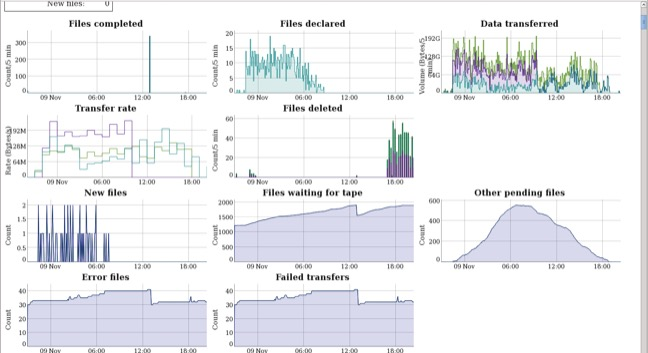
\includegraphics[width=0.5\textwidth]{./ReportImages/FTS.jpg}
  \caption{Monitoring of FTS copies}
  \label{fig:FTStoFermilab}
  
\end{figure}. 



\subsection {Future Work}
We clearly need to test data transfers originating from a disk on the EHN1 network - preferably from the pDUNE-SP and pDUNE-DP event data buffers. 

We need to converge on  the details of the metadata format and who writes it. It is currently agreed that this is provided by the DAQ/Online Group and they will write it. We hope the first test can be used to test this also. 

We need to move the FTS Virtual Machine from a private project OpenStack to the  DUNE OpenStack project. 

For the test the files moved to the DQM were declared to SAM since that is what FTS automatically does. We need to define the configuration of and move the files relevent to the DQM inbox without declaring them to SAM. From that point the DQM is responsible for their management.

We plan to clean this data challenge data set off of tape and SAM when the keep-up processing is completed.


\section {Data Quality Monitoring}
DC1 was an extremely useful exercise which helped to test and demonstrate the Data Quality Monitoring component
of the ProtoDUNE Single Phase offline system. Overall this was a success.

\subsection{Work-Up}

During the work-up to DC1 the week before, the following was validated
\begin{itemize}

\item The p3s infrastructure was pushed to utilize 1000 cores in CERN Tier-0 and kept that level of resource utilization for ~1hr
with realistic payloads
\item It was verified that p3s can accept jobs (means Apache and DB throughput) at ~100Hz rate

\end{itemize}
\noindent Technically this levels of throughput was not required in DC1 but it was considered important to know the system capability.
Characteristics of the HTCondor batch system in CERN Tier-0 were studied from the point of view of the DQM job sumbission and
execution.

In addition, automation for data discovery was created with periodic polling of the p3s ``inbox'' for new data according to a predefined pattern
and registration of these data for processing in the system. The p3s GUI was simplified and cleaned up. The current look of the p3s
dashboard screen is presented in Fig.\ref{fig:p3s_dash}.
\begin{figure}[tbh]
  \centering
  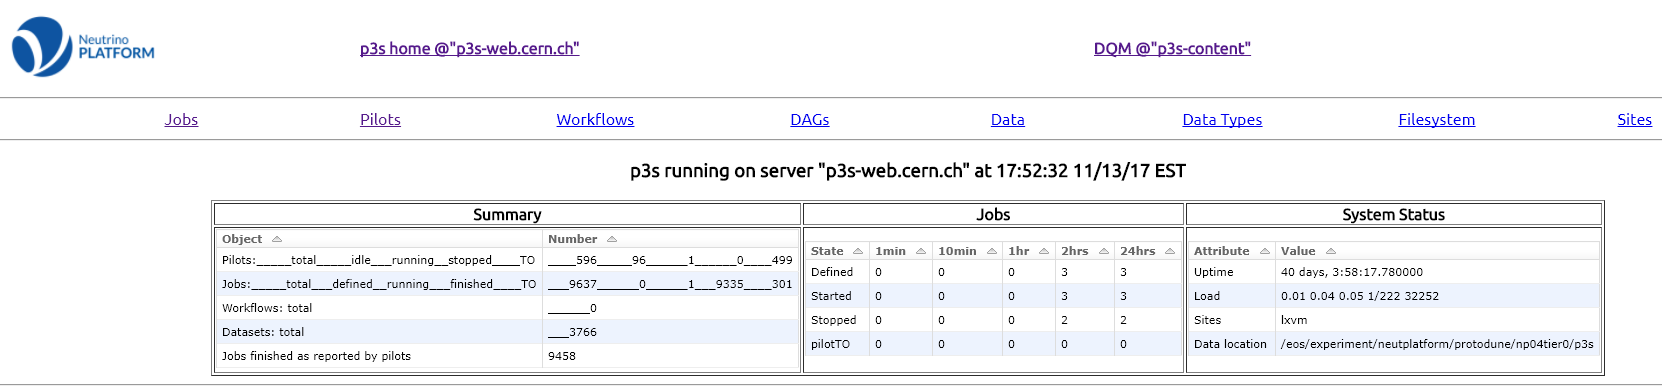
\includegraphics[width=1.0\textwidth]{./ReportImages/p3s_20171113_1.png}
  \caption{The p3s dashboard}
  \label{fig:p3s_dash}
\end{figure}

\subsection{Operation}
The p3s/DQM component of the Data Challenge remained operational throughout the testing period with virtually no human intervention.
It was monitored through its GUI and log files, and a few infrastructure issues that were discovered (see \ref{sec:p3s_issues}) were communicated
to CERN ITD. Processing kept up with the nominal data rate dictated by the rate of data transmission of DC1, with substantial headroom in
terms of the load on the p3s servers and also in terms of computing power available in CERN Tier-0.

\subsection{Payloads}
Three kinds of DQM payloads were used during DC1:
\begin{itemize}
\item A simple Event Display (channel vs time for each TPC section)
\item Purity Monitor (estimation of the electron lifetime based on a group of tracks)
\item CRT-to-TPC track match (tracking with Cosmic Ray Tagger, correlation with TPC)
\end{itemize}
\noindent These payloads performed without apparent failures. An example of the Event Display output
is presented in Fig.\ref{fig:evdisp}, demonstrating the functionality of this application.
\begin{figure}[tbh]
  \centering
  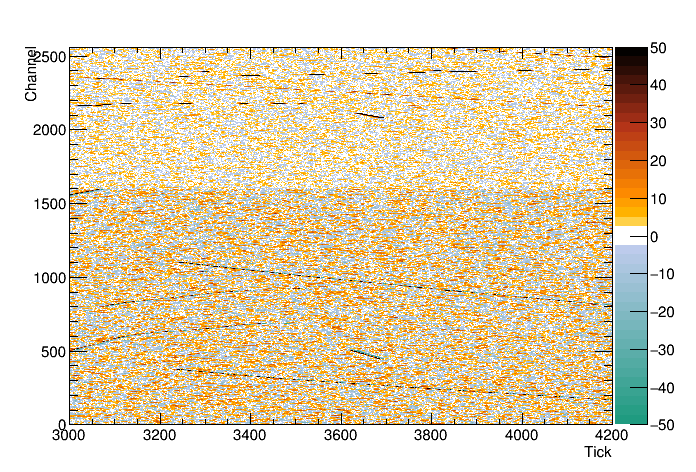
\includegraphics[width=0.6\textwidth]{./ReportImages/adcraw_evt33_ch0-2559.png}
  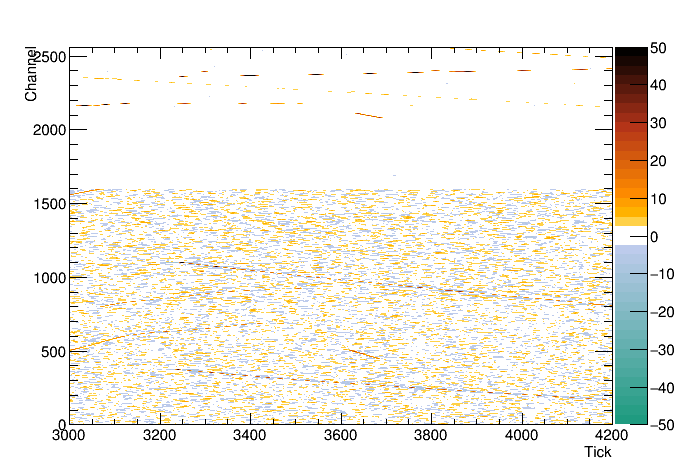
\includegraphics[width=0.6\textwidth]{./ReportImages/adcprep_evt33_ch0-2559.png}

  \caption{Event Display of same event before and after signal processing}
  \label{fig:evdisp}
\end{figure}

\noindent  A an auxiliary "presentation server" p3s-content.cern.ch
was used to serve the event display images and timestamped purity tables.

\subsection{Mode of Data Access}
The mode of data access by the payload jobs (both input and output) was FUSE mount of EOS.
Depending on the results of future data challenges this may provide enough performance and
stability for the \pd operations. If proven otherwise, migration to XRootD interface (such as \textit{xrdcp})
will be considered.

The presentation Web service was also accessing the DQM outputs via the FUSE mount which was 
soft linked to a directory included in the Apache server configuration. No problems were detected
with this setup during DC1.



\subsection{What we found}
\label{sec:p3s_issues}
A few potential problem areas were discovered when running with a large number of pilots:
\begin{itemize}
\item Indications of AFS clients losing connectivity in fraction of cases which also changes over time. Also reported in an unrelated situation by Robert. Results in the "bus error" message and loss of pilots - no good. Work in progress to find mitigation but not a show stopper
\item Condor vacating pilot jobs i.e. not respecting the required time limit. Filed a ticket. An error was found in the Condor cinfoguration, testing ongoing.
\end{itemize}

 
\subsection{What else to test/develop}

\begin{itemize}
\item Request from DRA to support full workflow mechanism in p3s - it has been implemented but not tested with realistic payloads.
\item The "basic metadata" issue - how to cross reference DQM and raw data potentially at sub-event level. Example - event display for an APA in a particular run/subrun/event. Or, account for purity data - list of events as reference to raw data.
Very different from the "Metadata" in the sense of the word we are typically using e.g. SAM etc. It is a product of DQM rather than of the data handling system.
\item Need "standard" JSON schemas and tools to facilitate this work for payload developers.
\item Beam Instrumentation payloads have not been tested in DQM.
\end{itemize}

\subsection{Summary}
If we had to use DQM p3s system tomorrow during data taking, it would likely meet many of its objectives, perhaps lacking somewhat in interfaces.
 
 

\section {Keep up Processing}

 \color{red} We will wait til the end of the current Keep Up processing tests/runs to complete/correct this section. Hope to get some more results to include.
 \color{black}

The Data Challenge 1 Keep Up Processing  included end to end testing of the offline processing infrastructure, physics payloads to be used for reconstructed simulation data in the upcoming monte carlo challenges, and declaration of output files back into the catalog and archival storage.  In order to decouple infrastructure issues from  payloads problems, it was agreed to split the Data Challenge into three phases and run the processing more than a week if needed:
\begin {itemize}

\item Phase 1: Simple "null" script
 Copies in input from the SAM dataset.  Sleeps for a well defined amount of time.  Renames the file and copies it out with appropriate metadata to the offline dropbox.
This stage is designed to completely decouple from ANY art or LarSoft dependancies or reconstruction code. 



\begin{figure}[tbh]
  \centering
  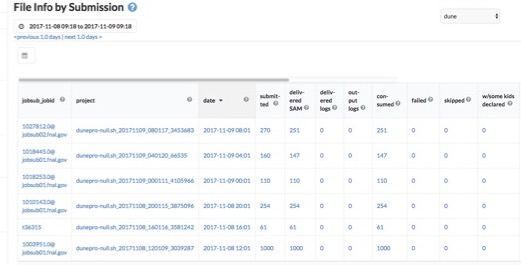
\includegraphics[width=0.8\textwidth]{./ReportImages/Phase1keepup.jpg}
  \caption{POMS Monitoring of Phase 1 of Keep Up Processing Jobs}
  \label{fig:keepupprocessingphase1}
\end{figure}


\item Phase 2: Simple art/Larsoft based "null" jobs
 ?Real art/Larsoft job, but one that does effectively nothing.  This stage is designed to identify and potential problems with the use of the framework and workflows, but NOT be dependent on a specific set of reconstruction algorithms.  
 This stage is ready to run but will not be run until the simpler null jobs have been throughly tested at scale.


\item Phase 3: Full payload art/Larsoft "mini-reco" jobs

 Run  a mini-reco processing using the configurations provided by Robert and Dorota. This stage will defer till stages 1 and 2 have been successful.

\end{itemize}

\subsection {Preparation}

POMS campaigns and configurations scripts are tested.
For each campaign, a keepup processing is setup to run every 4 hours (6 submission/24 hours).
At each submission, all new files coming in the input SAM dataset are processed.
The files are renamed and copied with appropriate metadata to the offline dropbox where an FTS instance is configured to copy them on tape (@FNAL and @CERN if requested).
POMS is also configured to automatically  recover:  ?- files that have not been consumed?- files from failed jobs.
Mergeana files as input of DC1 required particular care and additional tests.
Grid jobs submitted  without the additional layer of project.py required some more work but with the advantage of a better control of the entire workflow.

\begin{itemize}
\item Phase 1 
Copy in, then Copy out, with a 2 min sleep between them.
The keepup processing ran smoothly after several fine tunings.
A bug related to the input dataset (there was no control that input files were copied to FNAL) where found and immediately fixed.

\item Phase 2 
Copy in then  Copy out, using LarSoft executable where the algortihm code is just a 7 min sleep. It?s on going and running smoothly since last midnight.
The processing is monitored to identify problems and bottlenecks.

\item Phase 3
\color{red} to be added
\color{black}

\end{itemize}

\subsection {Sam Projects and File Copy Status}
Last SAM Project of Phase 2 (Submission @ 4am CST)

\href{http://samweb.fnal.gov:8480/station_monitor/dune/stations/dune/projects/dunepro-null_lar.sh_20171110_040116_3425472}{Sam Catalog}



\begin{figure}[tbh]
  \centering
  \includegraphics[width=0.5\textwidth]{./ReportImages/SamProjectsKeepupoutput.jpg}
  \caption{Monitoring of File Movement During Keep Up Processing}
  \label{fig:FTSKeepUPProcessing}
\end{figure}



\begin{figure}[tbh]
  \centering
  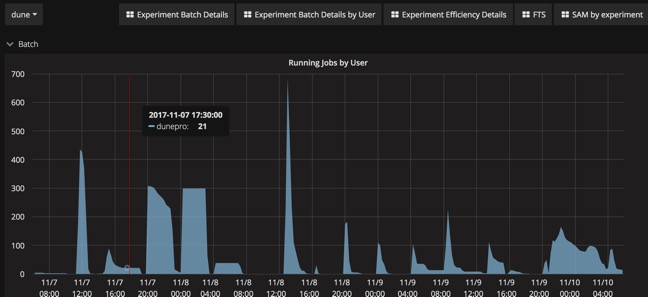
\includegraphics[width=0.5\textwidth]{./ReportImages/FIFEMonkeepup.jpg}
  \caption{Monitoring of Batch Jobs associated with Keep Up Processing}
  \label{fig:FIFEmon}
\end{figure}



\subsection {Summary}

DC1 ProtoDUNE SP has been a BIG step forward for next production processing.
The infrastructure for production processing is in place.
Many thanks to everybody who has contributed for this success.
Particular thanks to Marc Mengel and all POMS developers of SCD for their passionate work. Thanks to them our team has an excellent system for production and data processing.



\section {Beam Instrumentation}

Two parts of the beam instrumentation infrastructure were tested. The first is for sustained transfer data from an existing DIP (LHC) service at CERN to the IFBEAM database instance at Fermilab. The second is to ingest fake protoDUNE beam instrumentation data to the IFBEAM database and then read it back out into a data processing job using the LArSoft framework. 

 \color{red} Do Igor and/or Jon have any slides I can take from here or shall I just write up what we have in the various emails? 
 \color{black}


\subsection {Ingest from DIP Service}

All CERN data is currently stored as short-term data only.   Meaning the database will only retain it for a month.   We are leaving it like this until we start taking production, long-term, data.   As we near production, it will be very important that we know when to switch.  Even though this data is ?noise?, we would like to keep it running for testing purposes.
\subsection {Fake data test}
 This data is being stored as long-term stored under a different "event" to distinguish it from production.

\section {Collaboration Tools}
\begin {itemize}
\item SLACK Channel
We successfully used a data challenge slack channel to communicate ongoing work and issues encountered. 
\item  wiki monitoring links
We used a
\href {wiki.dunescience.org} page to link to monitoring and documentation information relevant to operations of the data challenge. 
\item physical and virtual rooms 
we were more or less successful in having  a regular meeting using zoom as part of the challenge. Since only Maxim travelled to CERN for this data challenge the use of a physical meeting room was less successful

\section {Input to the Data Challenge 2 Planning}

\begin{itemize}
\item Following the work on DC1 the hope is to have DC2 as a collaboration between ProtoDUNE Single Phase (NP04) and ProtoDUNE Dual Phase (NP02). 

\item DC2 will be a test of the full data flow, archiving and processing rate + some overhead to allow for contingency in cosmic ray and beam data volumes as well as event processing times. 

\item Event data files read out from the detector will be used.

\item It is clear that some operational effort is needed to keep the system flowing. DC2 should plan for and implement operations as if data taking was happening. 

\item There are some functions with "Single points of resource failure". We should try to obviate these for DC2 and ensure more than one person for each function is handling the operation/execution/debugging. All offline services should be running as "DUNE services" rather than in individuals areas or computers. 


\end{itemize}



\end{itemize}



\clearpage



\end{document}

%%% Local Variables:
%%% mode: latex
%%% TeX-master: t
%%% End:
\grid
